
\chapter{The Plan7 profile HMM architecture}

%%%%%%%%%%%%%%%%%%%%%%%%%%%%%%%%%%%%%%%%%%%%%%%%%%%%%%%%%%%%%%%%
%
\section{The core probability model}
%
%%%%%%%%%%%%%%%%%%%%%%%%%%%%%%%%%%%%%%%%%%%%%%%%%%%%%%%%%%%%%%%%

The \textbf{core model} is a generative probabilistic model of global
sequence alignment. It consists of match (M), delete (D), and insert
(I) states, plus a special begin state (B) and end state (E) as shown
in Figure~\ref{fig:plan7-core}.

\begin{figure}
\begin{center}
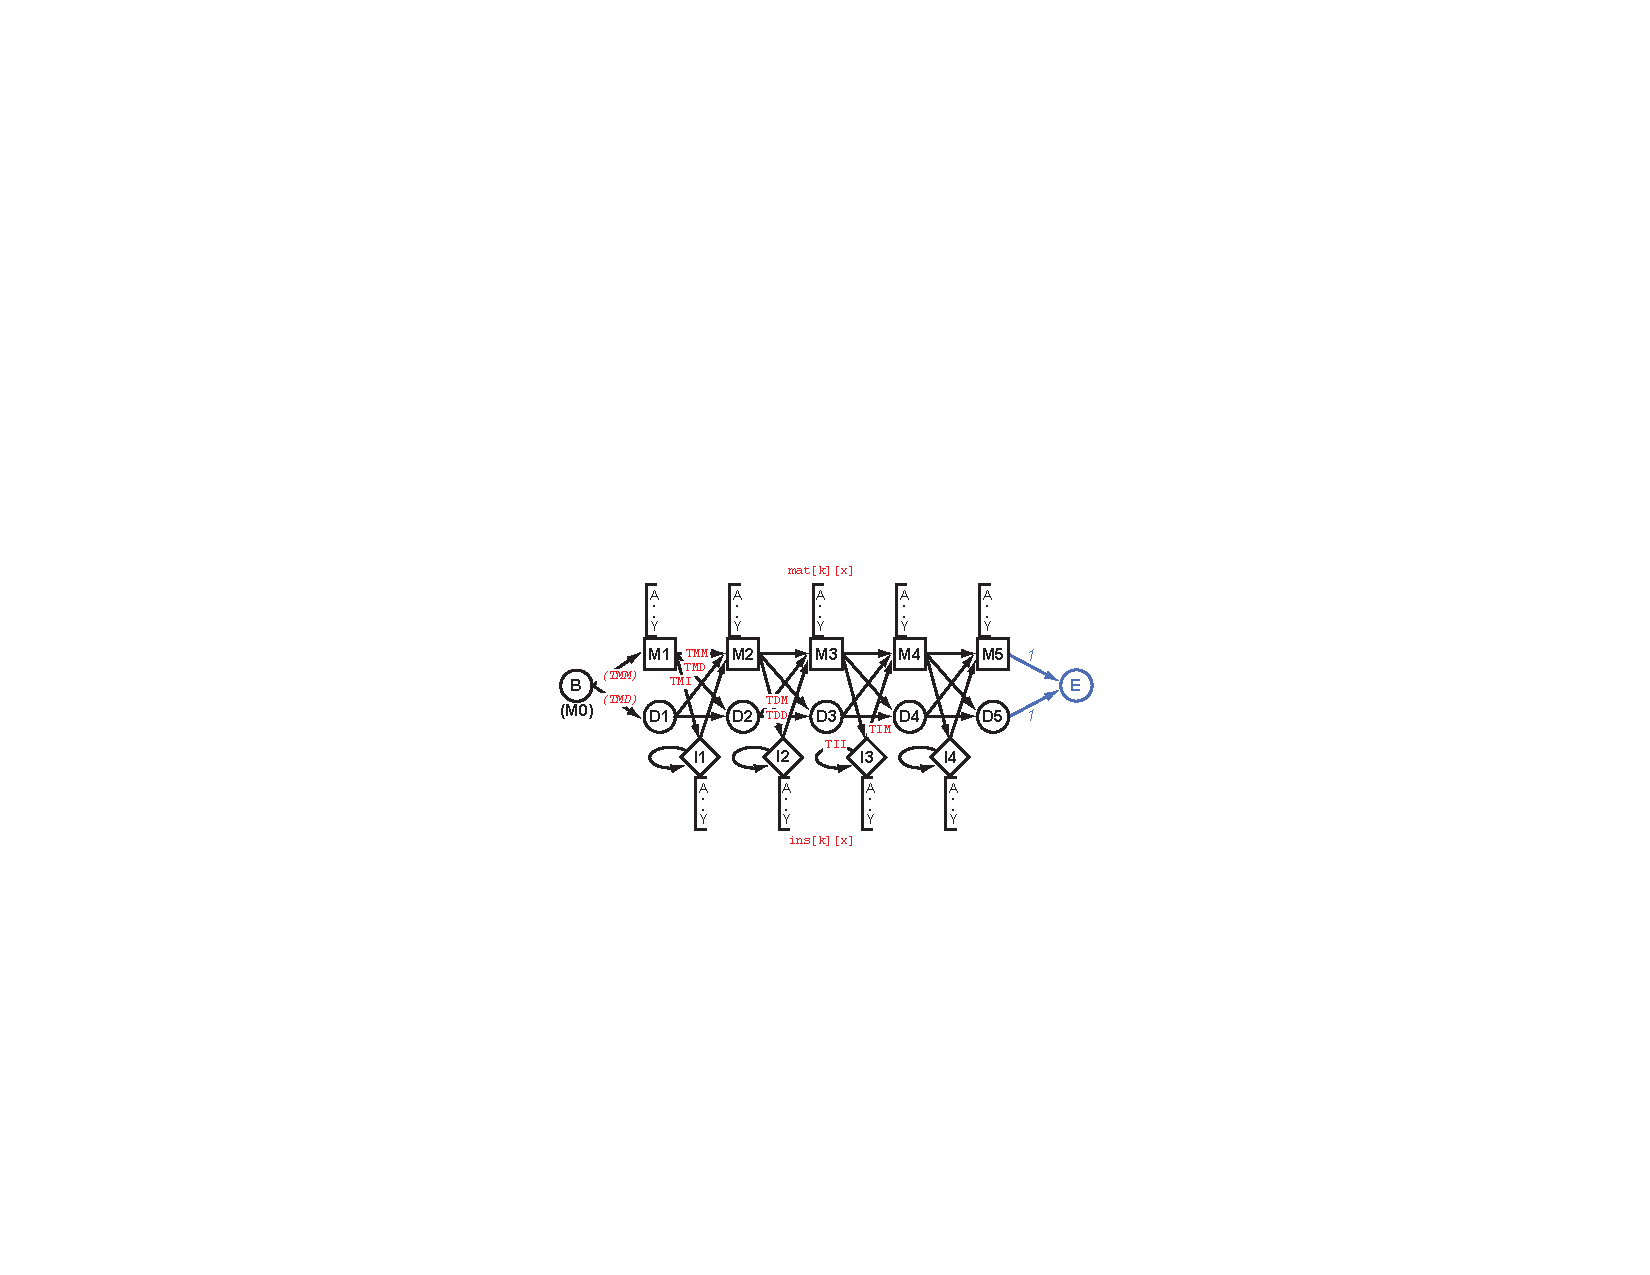
\includegraphics{figures/plan7-core}
\end{center}
\caption{The core probability model. Codes for the seven
transitions (\ccode{t[k][TMM]}, etc.) are shown in red.} 
\label{fig:plan7-core}
\end{figure}

The core model is implemented in the \ccode{P7\_HMM} structure in
\ccode{plan7.h}:

\input{cexcerpts/plan7_core}

Each consensus column $1..k..M$ of a multiple alignment is assigned to
one \textbf{node} consisting of a M, D, and I state triplet. The $M_k$
state generates a residue $x$ according to emission probabilities
estimated from consensus column $k$ with probability
\ccode{mat[k][x]}.  The $I_k$ state emits one or more residues $x$,
inserted between consensus columns $k$ and $k+1$, each with
probability \ccode{ins[k][x]}). The match and insert emission
distributions represent an alphabet of $K$ total residues, $K=4$ for a
nucleic acid model, and $K=20$ for a protein model. The $D_k$ state
is mute (that is, it does not emit a residue), allowing a residue in
column $k$ to be skipped (a deletion relative to consensus).

This design essentially follows the profile HMM architecture
introduced by Krogh \emph{et al.}  \citep{Krogh94}. The main
difference is that $D_k \rightarrow I_k$ and $I_k \rightarrow D_{k+1}$
transitions are omitted by HMMER. The Krogh/Haussler model has nine
transitions per node, whereas HMMER has seven. Internally, we call the
HMMER architecture ``Plan 7''. The seven transition probabilities for
node $k$ are stored in \ccode{t[k][p7\_TXX]}, where \ccode{XX} is one
of the seven possible combinations of M,D,and I
(Figure~\ref{fig:plan7-core}).

The begin state (B) is stored internally as match state 0 with two
transitions \ccode{t[0][p7\_TMM]} and
\ccode{t[0][p7\_TMD]}. \ccode{t[0][p7\_TMI]} is hardcoded to be zero.

The end state (E) is not explicitly represented in the core model.
Neither are the transitions of the final node $M$.  Transitions from
the final M,D states to E are implicitly 1.0.

All paths through the profile core (samples from $P(x, \pi \mid H)$)
must visit either a match or delete state in every position $k$.
Every residue $x_i$ in the emitted sequence is assigned to either a
match or an insert state.


%%%%%%%%%%%%%%%%%%%%%%%%%%%%%%%%%%%%%%%%%%%%%%%%%%%%%%%%%%%%%%%%
%
\section{The score profile}
%
%%%%%%%%%%%%%%%%%%%%%%%%%%%%%%%%%%%%%%%%%%%%%%%%%%%%%%%%%%%%%%%%

% Fragment below is from old plan7.h, comments on the HMM
\begin{cchunk}
 * 2. The "configured" model is the scoring form.
 *    It adds the S,N,B; J; E,C,T special states of the Plan7
 *    "algorithm-dependent" probability architecture.
 *    
 *    The S and T states are not explicitly represented anywhere.
 *    S->N is implicitly 1.0. 
 *    
 *    N,E,C,J transitions are set in xt[]. N,C,J emissions are implicitly
 *    equal to the null model emission probabilities, and these states emit
 *    on transition. 
 *    
 *    Entry into the model is controlled by begin[], which is a normalized
 *    prob distribution \sum_{k=1}^{k=M} t(B->M_k) = 1.0. Exit from the model
 *    is controlled by end[], which is not a probability distribution itself;
 *    rather, \sum_{x=MDI} t(M_k->x) + t(M_k->E) = 1.0. 
 *    
 *    A configured model has no D_1 or D_M state. A process called
 *    "wing retraction" is applied by the configuration functions, to
 *    eliminate the mute all-delete B->D_1...D_M->E path. Wing
 *    retraction requires altering the transition probabilities in the
 *    nodes. See modelconfig.c.
 *    
 *    Only two combinations of wing retraction and internal entry/exit
 *    are allowed. In sw/fs mode models, algorithm-dependent entry and
 *    exit probabilities partially trump wing retraction, so begin[]
 *    and end[] are unaffected, though other effects of wing
 *    retraction take place; in an alignment, all B->M_k and M_k->E
 *    begins and exits are interpreted literally as B->M_k and M_k->E
 *    transitions. In ls/s mode models, there is no algorithmic
 *    internal entry/exit probability, but wing retraction contributes
 *    data-dependent probability to begin[] and [end]; in an
 *    alignment, B->M_k and M_k->E internal begins/ends are
 *    interpreted instead as delete paths B->D1->...->D_k-1->M_k or
 *    M_k->D_k+1->...->D_M->E.  That is, internal entry and exit probs
 *    may only be *entirely* algorithm dependent (from configuration)
 *    or *entirely* data-dependent (from wing retraction of the core
 *    model), not a mixture of both. (The reason is that if they're a
 *    sum of the two, you can't correctly extract a Viterbi alignment
 *    from the sum.) When the configuration is using
 *    algorithm-dependent entry, the PLAN7_BIMPOSED flag is raised;
 *    when it is using algorithm-dependent exit, the PLAN7_EIMPOSED
 *    flag is raised.  (xref STL9/79, and modelconfig.c).
 *    
 *    After configuration, the core model is unchanged; xt, begin, end
 *    are set to probabilities; and bsc, esc, tsc, msc, isc, and & xsc
 *    are set to scores. In a configured model, tbd1 is not used (all
 *    entry into the model is controlled by B->M_k begins); D_1 and
 *    D_M don't exist and aren't used; D_M-1->M_M = 1.0 and M_M-1->D_M
 *    = 0.0 (because D_M doesn't exist); and all exits from the model
 *    are controlled by M_k->E ends.
 *    
 *    The PLAN7_HASBITS flag is up when the model is configured into
 *    score form.
 *    
 * hmmbuild creates a core model, then configures it, then saves
 * it. Both the core model and the configured model are saved.
 * 
 * Search programs like hmmpfam and hmmsearch read only the configured
 * score model, usually ignoring the core probability model.
 */

\end{cchunk}

% Another comment fragment, also from plan7.h P7_HMM
\begin{cchunk}
   *
   * Note that emission distributions are over possible alphabet
   * symbols, not just the unambiguous protein or DNA alphabet: we
   * precalculate the scores for all IUPAC degenerate symbols we may
   * see.
   *
   * Note the reversed indexing on msc, isc, tsc -- for efficiency
   * reasons. They're not probability vectors, so we can reorder them.
   * 
   * The _mem ptrs are where the real memory is alloc'ed and free'd,
   * as opposed to where it is accessed.  This came in with Erik
   * Lindahl's altivec port; it allows alignment on 16-byte
   * boundaries. In the non-altivec code, this is just a little
   * redundancy; tsc and tsc_mem point to the same thing, for example.
   * 
   * PLAN7_HASBITS flag is up when these scores are valid.
   */
\end{cchunk}

%%%%%%%%%%%%%%%%%%%%%%%%%%%%%%%%%%%%%%%%%%%%%%%%%%%%%%%%%%%%%%%%
%
\section{Internal score representation}
%
%%%%%%%%%%%%%%%%%%%%%%%%%%%%%%%%%%%%%%%%%%%%%%%%%%%%%%%%%%%%%%%%

Internally, profile scores are integers, calculated by rounding off
scaled log2-odds scores. The code refers to internal scores as SILO
scores (scaled integer log2-odds), as distinguished from bitscores,
which are the external representation as unscaled floating-point
values in bits.


